\section{Introduction}
Prompt adherence of text-to-image diffusion models is usually summarised by one score per image. Compositional failures, however, are constraint-specific: an object can be present while its colour is wrong, or two objects can be correct while their left--right order is not. If different constraints are resolved at different moments of the sampling trajectory, three practical consequences follow. Guidance strength that matters early may be wasted late; diagnostics that read early internal signals are forecasts for some constraints and read-outs for others; and a pooled adherence score can hide both effects.

Prior work establishes that denoising stages control different image properties \citep{patashnik2023mixing,zhang2023prospect,balaji2022ediffi,li2024critical}, that guidance can be restricted or scheduled over time \citep{kynkaanniemi2024interval,sadat2024cads,dynamiccfg2025}, and that cross-attention carries information about objects and attributes that can be read and steered \citep{hertz2023p2p,tang2023daam,chefer2023attend,epstein2023selfguidance}. We therefore do not claim that the general idea of stage-dependent generation is new. Our questions are narrower and measurement-first:
\begin{enumerate}
\item \textbf{When} does each constraint type (presence, count, colour binding, spatial relation, relative size) stop depending on the remaining randomness of the trajectory? We answer with an interventional, chance-corrected persistence curve rather than with an observational signal.
\item \textbf{What does CFG change?} Does a larger guidance scale move persistence earlier, once the higher seed-to-seed agreement it induces is accounted for?
\item \textbf{Can attention tell?} Does the step at which cross-attention stops changing track the interventional measurement?
\item \textbf{Is the timing usable?} Does a two-level guidance schedule whose switch step is read off development-set measurements keep adherence while raising diversity, and does it beat the same mean guidance applied in reverse order?
\end{enumerate}

\paragraph{Contributions.}
\begin{enumerate}
\item[(i)] An interventional, chance-corrected measurement of restart persistence per constraint type, with two re-noising probes and a closed-form stress test for judge error (Section~\ref{sec:methods}).
\item[(ii)] A controlled scene-graph benchmark with counterfactual variants and a factorial size family, scored by a judge whose blinded human audit decides which constraint types may carry claims (Sections~\ref{sec:benchmark}--\ref{sec:evaluation}).
\item[(iii)] Commitment-Aligned Guidance (CAG), tested against constant, reversed and matched-mean schedules under a signed pre-registration, with every gate reported whether it passed or failed (Sections~\ref{sec:methods} and~\ref{sec:resDEV}).
\item[(iv)] On the available test shards, an account of what survives: the guidance effect on timing, its sensitivity to the judge, the failure of commitment times to transfer, the dose explanation of CAG's diversity gain, and what saved cross-attention maps add to the restart measurement (Sections~\ref{sec:resPARTIAL}--\ref{sec:resATTN}).
\end{enumerate}

\paragraph{Findings in brief (partial test split, exploratory).}
\begin{itemize}
\item Stronger guidance makes object presence persistent earlier, with $t_{50}(w{=}15)-t_{50}(w{=}2)=\rbHdReg$ of 40 steps. This is the only registered rule that passed. The effect is not an artefact of the chance correction or of the full-resample offset. It does assume that the presence judge's errors are not independent across seeds.
\item Cross-attention moves in the same direction: higher guidance separates the object nouns and makes their attention stabilise earlier. Objects that are eventually missed have diffuse, overlapping attention from the first steps.
\item Attention stabilisation does not order the constraint types the way persistence does. Its binding signal follows object layout, not colour assignment.
\item Commitment times measured on the development split did not transfer to the test scenes, so CAG switched guidance down before binding had settled. CAG was not non-inferior to constant guidance, and its diversity gain is explained by its lower mean guidance.
\end{itemize}
We use the operational term \emph{restart persistence}; we do not claim that the model ``decides'' in any cognitive sense. Figure~\ref{fig:concept} summarises the probes and the schedule.
\begin{figure}[t]\centering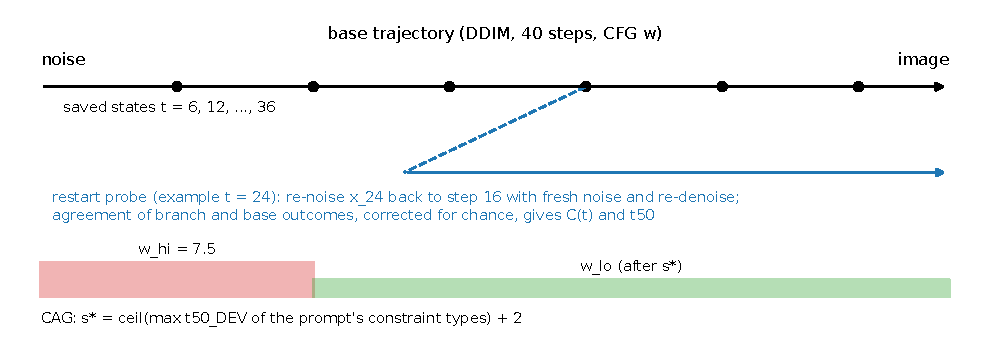
\includegraphics[width=\linewidth]{figures/fig_concept.pdf}
\caption{\textbf{Conceptual diagram} (not data). Top: a 40-step DDIM trajectory with saved states. Middle: the restart probe re-noises a saved state to an earlier step with fresh noise and re-denoises; agreement of branch and base outcomes, corrected for chance agreement between independent seeds, gives $C(t)$ and $t_{50}$. Bottom: CAG applies $w_{hi}$ until a prompt-specific switch step $s^\star$ derived from development-set $t_{50}$, then $w_{lo}$.}\label{fig:concept}\end{figure}
